\documentclass[border=5pt]{standalone}

\usepackage[T1]{fontenc}
\usepackage{garamondx}
\usepackage[garamondx,cmbraces]{newtxmath}
\usepackage{tikz}
    \usetikzlibrary{arrows,decorations}

\tikzset{%
    queue/.pic={%
        code{%
            \node (rect) at (38.5mm, 10mm) {};
            \draw[thick] (0, 0) -- ++(40mm, 0) -- ++(0, 20mm) -- ++(-40mm, 0);
            \foreach \val in {0, ..., #1}{%
                \draw[thick] ([xshift=-\val*5mm] 40mm, 20mm) -- ++(0, -20mm);
            };

            \foreach \val/\lab/\size in {%
                0/1/\scriptsize,
                1/2/\scriptsize,
                3/c-1/\tiny,
                4/c/\scriptsize%
            }{%
                \node[draw, circle, thick, minimum size=9.5mm] (\lab)
                    at (55mm, 29mm - \val * 9.5mm) {\size$\lab$};
                \draw[-latex, thick] ([xshift=3mm]rect.east) -- (\lab.west);
            };

            \node at (55mm, 11mm) {$\vdots$};
            \node at (5mm, 10mm) {$\cdots$};
        };
    },
    myarrow/.style={%
        line width=2mm,
        draw=gray!50,
        -triangle 60,
        postaction={draw=gray!50, line width=4mm, shorten >=6mm, -},
    },
    double -latex/.style args={#1 colored by #2 and #3}{%
        -latex,
        line width=#1,
        #2,
        postaction={%
            draw,
            -latex,
            #3,
            line width=(#1)/3,
            shorten <=(#1)/4,
            shorten >=4.5*(#1)/3
        },
    },
}

\begin{document}

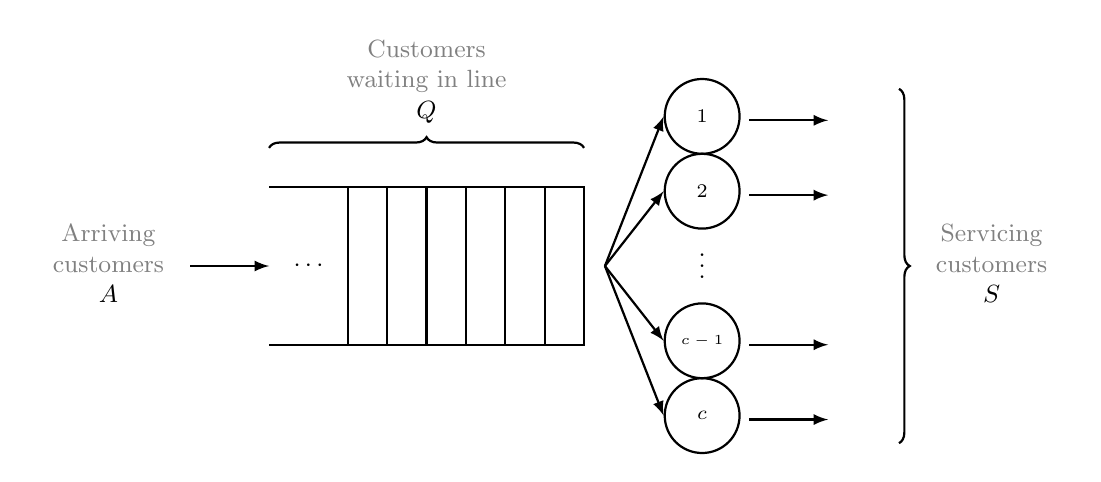
\begin{tikzpicture}

    \small
    \path (0, 0) pic {queue=6};

    \draw[-latex, thick] (-1, 1) to node[left, pos=0] {%
        \color{gray}
        \begin{tabular}{c}
            Arriving\\
            customers\\
            \color{black}\(A\)
        \end{tabular}
    } (0, 1);

    \draw[decorate, decoration={brace, amplitude=1ex}, thick]
        (0, 2.5) -- ++(4, 0) node[midway, above=1ex] {%
            \color{gray}
            \begin{tabular}{c}
                Customers\\
                waiting in line\\
                \color{black}\(Q\)
            \end{tabular}
        };

    \foreach \val in {-1, 0, 2, 3}{%
        \draw[-latex, thick] (6.1, \val * 9.5mm) -- ++(1, 0);
    };

    \draw[decorate, decoration={brace, amplitude=1ex}, thick]
        (8, 3.25) -- ++(0, -4.5) node[midway, right=1ex] {%
            \color{gray}
            \begin{tabular}{c}
                Servicing\\
                customers\\
                \color{black}\(S\)
            \end{tabular}
        };

\end{tikzpicture}

\end{document}
